\documentclass[12pt,oneside,justify]{book}

\usepackage[utf8]{inputenc}
\usepackage{mathptmx}
\usepackage{geometry}
\usepackage{fancyhdr}
\usepackage{tocloft}
\usepackage{titlesec}
\usepackage{textcomp}
\usepackage{pdfpages} 
\usepackage{graphicx}
\usepackage[magyar]{babel}
\usepackage{t1enc}
\usepackage{indentfirst}
\usepackage[shortcuts]{extdash}
\graphicspath{ {images/} }
\usepackage[
backend=biber,
]{biblatex}  % irodalomjegyzék

\titleformat{\chapter}{\normalfont\huge}{\thechapter.}{20pt}{\huge} % egyedi chapter szöveg

\geometry{
	a4paper,
	lmargin=3cm,
	tmargin=3cm,
	bmargin=3cm,
	rmargin=2cm
}

\fancyhead
\fancyfoot
\pagestyle{plain} % oldalstílus
\pagenumbering{arabic} % oldalszámozás 

\renewcommand{\headrulewidth}{0pt}
\renewcommand{\contentsname}{Tartalomjegyzék} % tartalomjegyzék átnevezés
\renewcommand{\listfigurename}{Ábrajegyzék} % ábrajegyzék átnevezés
\renewcommand\cftchapaftersnum{.} % chapter szám utáni pont
\renewcommand\cftchapdotsep{\cftdotsep} % chapter, és irodalomjegyzék szöveg utáni pontok
\newcommand{\sectionbreak}{\clearpage} % címsorok új oldalon


\addbibresource{bibliography.bib}

% help section - to be deleted

% \chapter{Második bekezdés}
% \section{másik bekezdés 2 szintű}
% \subsection{First Subsection}
% \paragraph{az}

% Ezt idéztem \cite{AzureFundamentals}

% \noindent // bekezdés első sorának  nem indentálása

% end help section

\begin{document} 

\includepdf{outer_cover.pdf}
\includepdf{inner_cover.pdf}

\tableofcontents

\chapter{Virtualizációról}

A számítógépek már a kezdetekben is annyira erősek voltak, hogy átlagos felhasználási módokkal nem lehetett teljesen kiaknázni a számítási teljesítményt vagy a tárkapacitást.
Ennek a problémakörnek a megoldására az igény az 1960-as évek közepén kezdett megnövekedni. 
Az akkori rendszerek single user, single application módban voltak képesek működni. 
Ez annyit tett, hogy a felhasználónak, ha egyszerre több folyamat futtatására volt szüksége, akkor annyi számítógépet kellett üzemeltetnie. 
A két éllovas az MIT és az IBM volt, az első kész megoldást azonban az IBM szállította. 
Az MIT-n akkor nem jól mérték fel a feladat jelentőségét, így nem szenteltek neki kellő figyelmet és elvesztették vezető szerepüket. 
Az IBM megoldásában egy specializált mainframe rendszert használtak, ahol a felhasználók párhuzamosan tudták futtatni a saját programjaikat.
A felügyeletre pedig egy parancssor állt rendelkezésre.
Ez azért volt nagy előre lépés, mert így a felhasználók egymástól elszeparált módon dolgozhattak.
Ez volt az első lépcső a virtualizáció mai formája felé.

A virtualizáció nem csupán az optimálisabb erőforrás elosztáshoz volt szükséges. 
A minden folyamatra külön kiszolgáló fenntartása komoly feladatok elé állította az üzemeltetésüket végzőket. 
A szerverek magas száma miatt nagy méretű adaközpontokat kell építeni, amelyekben a megfelelő körülményeket fenntartani nagyon költséges. 
A sok különböző szerver üzemeltetése, adminisztratív szempontból sem kisebb feladat. 
A kezdeti rendszereket nem lehett távolról egyszerűen vezérelni. Léteztek ugyan KVM megoldások amelyekkel limitáltan el lehetett végezni a távoli vezérlés bizonyos lépéseit, de már például a telepítéshez - főleg ha annak fizikai adathordozóról kellett megtörténni - szükséges volt a fizikai hozzáférés. 
A virtualizációs megoldások terjedésének köszönhetően, össze lehet fogni nagyobb csoportokba a szervereket. 
Aztán ezek felett a csoportok felett lehet definiálni az úgynevezett virtuális gépeket, amelyek osztoznak az erőforrásokon és a virtualizációs megoldástól függően akár mozoghatnak is a fizikai gépek között úgy, hogy a munkafolyamat nem szakad meg.

A fejlesztések azonban nem álltak le és megindultak a kutatások az alkalmazás virtualizáció irányába. 
Ezen irányú törekvések eredménye lett az egykori Sun Microsystems nevet viselő vállalat fejlesztése a Java. 
A Java nyelv legnagyobb előnye és egyben hátranya is, hogy bármely gépen elfut amelyen van Java Runtime Environment (JRE). 
A JRE felel azért, hogy az alkalmazások egy külön virtuális gépben fussanak az operációs rendszeren belül. 
Így az univerzális nyelven megírt alkalmazások teljesen szeparált, de előre jól tervezhető módon futnak szinte bármilyen hardveren és operációs rendszeren.

Jelenleg a virtualizációs megoldásokat már a biztonság fokozására használják, ezt bővebben a gyártóspecifikus részben taglalom.

\section{On-Premises rendszerek}

\subsection{Microsoft Hyper-V\texttrademark}

A Microsoft Hyper-V története egészen 1997-ig nyúlik vissza, amikor is még a technológiát a Connectix nevű cég birtokolta. 
Az első verziós kiadása a Virtual PC-nek még Macintosh platformra készült el. 
Ezt követte 2001-ben az első Windowsos megjelenés. 
A Microsoft miután egyértelművé vált, hogy az üzleti felhasználóknak szükségük van virtualizációs megoldásokra 2003-ban megvásárolta a Virtual PC-t és az akkor még nem kiadott Virtual Servert a Connectix-től. 
A microsoft folytatta mindkét termék fejlesztését. A Virtual PC több frissítésen is átesett mígnem a Hyper-V lenem váltotta 2008-ban. 
A Virtual Server a kezdetektől fogva a szerver operiációs rendszerek és az üzleti felhasználók igényeinek megfelelően lett fejlesztve. 
Olyan nem elhanyagolható különbségekkel, hogy a szerver verzión már a kezdetektől fogva az NTFS akkori szabványának megfelelő 2TB-os méretet ki lehetett használni, míg a Virtual PC-n 127GB volt a maximum. 
A 127GB-os limit a korabeli merevlemezek kialakításából adódott, hiszen a konszumer lemezekben nem volt kontroller így az operációs rendszer nem cellák alapján címezte a lemezt hanem a geometriáját felhasználva térben írta le a helyet, ezt kellett használnia a virtuális lemezeknél is a VPC-nek, hogy az operációs rendszerek működőképesek maradhassanak.

A Microsoft Hyper-V ezzen a néven először a Windows Server 2008 operációs rendszerben debütált. 
Megjelent belőle ugyanekkor egy ingyenes verzió is Hyper-V Server néven, amely nem volt más mint egy Windows Server 2008 Core edition, a Hyper-V role-al előtelepítve, míg a többi Role letiltásra került.
A Hyper-V most már minden mai Windows kiadásban rendelkezésre áll. A kezdeti limitált képességeit az újabb verziókkal kibővítette és most már teljesen valós opció a többi nagy virtualizációs platform mellett. 

A későbbiekben bemutatom azon funkcióit amelyek a virtualizált rendszereknél elengedhetelenek és amelyeknek köszönhetően a stabilitás, biztonság, és a skálázhatóság megoldható a Microsoft saját rendszerével annélkül, hogy megvásárolható opció lenne, mint más gyártóknál.

\subsubsection{Nano Server}

A Windows Server 2016-os kiadásával debütált és legfőbb célja a minimális overhead melletti üzemeltetés. 
Ezen kiadás telepítés utáni öszemérete 800MB, grafikus felhasználói felülete nincs így távoli managementre lett tervezve.
A kis mérete miatt nagyon gyorsan telepíthető, kevesebbszer kell patchelni, a szokásos havi iterációk helyett negyedéves ütemezéssel. 
Ezzel a rendelkezésre állása megnőtt. 
Ugyan korlátozott funkciókra használható, de azokon a területeken nagyon fontos előrelépés. 
Nano Server lehet 
\begin{itemize}
	\item Compute Node egy clusterben
	\item Scale-Out file serverben Storage Host
	\item DNS szerver
	\item IIS Webszerver
	\item Containerben futó alkalmazás gazdagép
\end{itemize}

\subsubsection{Deduplikáció}

A Microsoft a Windows Server 2012 szerver verzióban jelentette be a Deduplikációt. 
A deduplikáció az a folyamat amely feldolgozza az engedélyezett lemezek tartalmát és egyező adatblokkokat csak egyszer tárol le. Az ismétlődő blokkok esetén már csak referenciákat hagy. 
Ezzel a megoldással nagyon jó hatásfokkal lehet tárolóhelyet megtakarítani. 
A legjobban deduplikálható adatok a Virtualised Desktop Infrastructure -- későbbiekben VDI rendszerek -- amelyek esetén az operációs rendszer a hozzátartoztó frissítési csomagok, a feltelepített alkalmazások alapfáljai többnyire minden rendszeren megegyeznek. 
Amennyiben a virtuális gépeken nagyon kevés egyedi fájl és telepített alkalmazás található úgy a deduplikációs ráta elérheti akár a 80\%\=/ot is, ahogy az a \ref{fig:deduplication_ratio}. ábrán is látható.

\begin{figure}[ht]
\centering
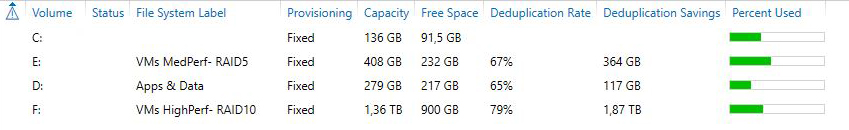
\includegraphics[width=0.8\textwidth]{deduplication-ratio-sample}
\caption{Deduplikációs ráta egy Hyper-V szerveren amelyen teszt szerverek futnak virtuális gépekként}
\label{fig:deduplication_ratio}
\end{figure}

\subsubsection{Cluster Rolling Upgrades}

A klaszterbe fűzött hostokon futó operációs rendszert lecserélni nem volt egyszerű művelet, mert a Windows nem támogatta egy az egyben a frissítést. Így egy kerülő megoldást kellett használni az In-Place upgradehez. Egy ilyen folyamat a következő lépésekből áll:
\begin{enumerate}
	\item Egy node a régi klaszterből való evakuálása
	\item Az evakuált node újratelepítése az új operációs rendszerrel
	\item A frissen telepített node\=/dal, egy gépből álló klaszter létrehozása, a közös storage konfigurálása.
 	\item A virtuális gépek migrációja a két cluster között.

Mivel a Hyper-V nem támogat direkt cluster-to-cluster migrációt, ezért a virtuális gépeket először ki kell venni a magas rendelkezésre álló gépek közül. Ilyenkor azon a node\=/on tudnak csak létezni ahol akkor voltak mikor megváltoztattuk a rendelkezésre állás szintjét.
	\begin{itemize}
		
		\item VM eltávolítása a magas rendelkezésre állású gépek közül
		\item VM migrációja az új clusterre
		\item VM konfigurálása magas rendelkezésre állásúvá
	\end{itemize}
	\item Amikor már minden gépet lemozgattuk a következő telepítésre váró gazdagépről, akkor azt lehet újratelepíteni és hozzáadni az új clusterhez.
	\item Amikor már csak egy node van a régi clusterben de már nincs rajta több virtuális gép, azt a cluster-t el kell pusztítani, és a gépet újratelepítve be lehet kötni az új clusterbe.
\end{enumerate}

A Server 2016-ra történő frissítés során a clusterek lehetnek mixed módban. Azaz lehet bennük 2012 R2 és 2016-ot futtató host is. A mixed mód alatt a cluster a 2012 R2-es funkciókészletet használja, amikor befejeződik minden node\=/on a frissítés, onnantól használhatóvá válnak az új lehetőségek is. Az előzőekben taglaltam, hogy milyen lépések szükségesek ahhoz, hogy rolling upgrade nélkül el lehessen végezni a frissítést kiesés nélkül. 
Ugyanaz a folyamat rolling updrage használatával:
\begin{enumerate}
	\item A kiválaszott node\=/on találató VM-ek evakuálása.
	\item A node újratelepítése 2016-al.
	\item Az újratelepített node visszacsatlakoztatása a cluster-be. 
	\item Ugyanezen lépések ismétlése míg az utolsó node is újratelepítésre nem kerül.
\end{enumerate}

A 2016-ra való frissítést nagyon hamar fogják erőltetni az üzemeltetők, mert a 2016-os Hyper-V a virtuális gép leállítása nélkül képes a kiosztott virtuális processzor magok számának, az allokált memória növelésére és csökkentésére. Eddig ezekhez mindig le kellett állítani a guest gépet. 

\subsubsection{Scale-Out file server}

Világunkban a tárolandó adatmennyiség egyre csak növekszik. Léteznek olyan termékek melyek kimondottan csak az adattárolásra specifikálódtak pl. NetApp Appliances, DellEMC Compellent vagy XtremeIO rendszerei. Ezek nagy telljesítményt tudnak nyújtani az üzemeltetést segítő plusz funkciók mellett, ám ezek bekerülési költsége nagyon magas.
A Microsoft erre a feladatkörre fejlesztette ki a Storage Spaces technológiát és az arra épülő Scale-Out File Server\=/t.
\newline
A Storage Spaces technológia lényege, hogy sok, akár különböző lemezt tudjon összefogni egy logikai egységgé, amely fölött virtuális meghajtókat definiál. Ezen virtuális meghajtók nagyon hasonlítanak a RAID tömbök felett definiált meghajtókra, hiszen ugyanúgy meg kell adni a hibatűrését.  A Storage Spaces nagy előnye, hogy képes a virtuális meghajtókat több különböző típusú lemezből elkészíteni. Például létrehozhatunk SSD cache-l megtámogatott virtuális meghajtót, amely esetén az adatok mozgatását a rendszer végzi, az alkalmazások és a felhasználók számára teljesen transzparensen, hasonló módon mint ahogy az operációs rendszerek a memóriát lapozzák.

A Scale-Out File Server képessége, hogy 2 és 8 node közötti failover cluster-t hoz létre amelyen a megosztott meghajtók ugyanúgy működnek mint a Hyper-V Failover Clusterben a virtuális gépek. Tehát ha valamelyik storage node\=/ot le kell állítani akkor az ő álltal birtokolt megosztások átkerülnek egy másik node\=/ra, a lemezei vezérlését pedig szintén egy másik node veszi át.

\subsubsection{Storage Spaces Direct}

Windows Server 2016-al debütált megoldás, amely az alacsonyköltségvetésű klaszterek kiépítését segíti elő. A Failover klaszterek alap követelménye, hogy legyen egy közös tárolóhely ahol virtuális gépek lemezfáljai és a konfigurációs fáljuk tárolva van. Így amikor a virtuális gépet mozgatni kell a node\=/ok között akkor csak az aktuális memória állapotot kell átmásolni az új hostra és már mehet is tovább a munka. 
A Storage Spaces Direct lényege, hogy a hostok saját beépített lemezeiket használják. A rendszer majd később ezekből a lemezekből készít egy disk poolt, és azon definiálhatóak a tényleges meghajtók. Ezek a meghajtók a kialakítás miatt hibatűrőek, és az adatok úgy vannak elosztva, hogy a munkafolyamat akkor is tud tovább menni, ha az egyik cluster node leáll vagy leszakad a hálózatról.
A rendszer bármikor bővíthető mert a háttérben a SoFS adja a megoldást.

\subsubsection{Storage Replica}

Windows Server 2012R2-től elérhető funkció a Hyper-V replica. A replikációnak köszönhetően fenn lehet tartani egy teljesértékű másolatát egy virtuális gépnek vagy gépek halmazának. A replikációs intervallum 1 óra és 5 perc között konfigurálható, azaz ha az eredeti gép megáll vagy valamilyen probléma adódik vele, akkor a replikát el lehet indítani ezáltal maximum a konfigurált replikációs időtartamnyi munkafolyamat elvesztésével kell számolni. Ezzel a megoldással jól lehet Off-Site backup-okat készíteni, akár Azure Cloud-ba is.

A Storage Replica az Hyper-V Replica másolata, csak itt a SoFS meghajtóit lehet biztonságosan tükrözni egy másik példányra.

\subsubsection{Virtual Network}

A Hypervisor-ok már a kezdetektől fogva képesek voltak a virtuális hálózatok kezelésére. Továbbá képesek a saját fizikai hálózati portjukon keresztül több különböző forgalmat lebonyolítani, plusz a szerver rendszerekben rendelkezésre áll a fizikai hálózati kártyák egy csoportba való összefogása. Ugyan így az átviteli sebességet nem tudjuk agregálni, tehát hiába fogunk össze 4db 10Gbps hálózati linket akkor nem tudunk egyszerre kifelé 40Gbps-el kommunikálni egy adott host felé, ám ha egy időben 4 különböző hostal szeretnénk a kommunikációt végre hajtani akkor az egyéni linkek maximális sebességét tudjuk hozni. 

A virtuális hálózatoknak köszönhetően a hostokon vagy clustereken belül tudunk privát alhálózatok létrehozni amellyel az adatközlést még biztonságosabbá és szeparáltá lehet tenni.

\subsection{VMWare ESX \textsuperscript{\textregistered}}


\subsection{Oracle\textsuperscript{\textregistered} VM}


\section{Cloud megoldások}
\subsection{Microsoft Azure}
\cite{AzureFundamentals}


\subsection{VMWare Cloud}


\subsection{Oracle Cloud}


\section{Platformok összehasonlítása}


\chapter{Esettanulmány}

A dolgozat megírásakor nem állt rendelkezésre, olyan alany akinek az esetét fel lehetett volna dolgozni, így egy feltételezett igénylőt alkottam meg. 

Az igénylőt a manapság igen divatos Start-Up cégek mintájára alkottam meg. Egy ilyen cégnél fontos, hogy minél alacsonyabb legyen a kezdeti kiadás mértéke. Számukra ezért lehet előnyös egy hosting céghez fordulni. A webfejlesztéssel foglalkozó személyeknek úgy sem idegen az ilyesféle megoldás. Az igénylő a megkeresésekor elmondta még, hogy szeretnének mobil alkalmazás fejlesztéssel, és Android egyedi rom-ok gyártásával foglalkozni. De szeretnék, ha mindezt egy központi verziókövető rendszerben tudnák tárolni. 

\section{Igényfelmérés}
Az ilyen jellegű munkáknál is nagyon fontos az igényfelmérés. Egyrészről szükséges ahhoz, hogy a megrendelő a végén úgy érezze, hogy mindent megkapott amit szerett volna. Másrészről a szolgáltatót is fedezi, mert egy korábban megállapított és közösen elfogadott követelmény rendszernek megfelelő rendszert ad át.
\newline
\newline
Az igényfelmérés több lépcsőből áll. 
\subsubsection{Elbeszélgetés}
Ez az első lépése a követelmények felmérésének. Ez a szekció egyszer történik meg, ilyenkor a megrendelő és a szolgáltató egy embere - akik nem feltétlenül rendelkeznek technikai tudással - egy megbeszélés során, összeszedik, hogy mit szeretnének elérni. 

\subsubsection{Technikai feltételek meghatározása}
Ez a feltárási művelet akár többször is megtörténhet még mielőtt elérnék a végső állapotot. Ebben a szekcióban már technikai megbeszéléseknek is meg kell történni. 
Meg kell határozni a következő tényezőket:
\begin{itemize}
	\item Operációs rendszer meghatározása - ha lényeges a keretrendszer miatt
	\item A keretrendszer kiválasztása
	\item A hardver specifikációnak méretezése - fejlesztés, teszt, és élő rendszerekre
	\item A front-end és back-end rendszerek meghatározása
	\item Egyéb kapcsolódó szolgáltatások feltárása 
\end{itemize}


\section{Ajánlat}


\section{Migráció cloudba}


\chapter{Esettanulmány háttércég}

\section{Architektúra}

Architektúrális szempontból Intel alapú szervereket használtam. A fejlesztői és tesztelői környezet alapját 2 db Dell PowerEdge R710-es szerver adta. A szerverek a munka ideje alatt egyenként 2 db Intel{\textsuperscript{\textregistered}} Xeon{\textsuperscript{\textregistered}} E6545 processzorral (6 mag 12 HT szál), 96 GB DDR3 ECC RAM-al, 2x64 GB Rendszer lemezekkel illetve 2x136 GB adatlemezzel volt ellátva. A kettő szerver egy failover clusterben üzemelt. A rendszer és az adat lemezek RAID1-ben üzemeltek az adatvesztés megelőzése és a magas rendelkezésre állás biztosítása érdekében. Az adatlemezek mérete sosem volt gond a Windows Deduplikációs megoldása miatt.


A rendszereinket központilag nem menedzselt, de egységes alapkonfigurációval látjuk el annak érdekében, ha az ügyfélnek segítségre lenne szüksége. 


A megépített rendszerben használt alapkonfiguráció:
\begin{itemize}
	\item Processzor: 2 mag
	\item Memória: dinamikus memória 1 GB minimum, 2 GB induláskor, 4 GB maximum.
	\item Háttértár: 64 GB Operációs rendszer lemez, 32 GB Adat lemez
	\item Hálózati kártya: 1 DB a megrendelő rendszerinek a belső hálózatán
	\item Operációs rendszer: Windows Server 2012 R2
\end{itemize}

\subsubsection{A mester image használata}

A mester image előállítása nagyban meggyorsítja a megrendelt rendszerek üzembehelyezését. Alapvetően két nagy irányzatot érdemes megemlíteni ezen megoldások terén. 

Az első megoldás amikor már egy teljesen kész rendszert tartalmazó de sysprep-elt virtuális merevlemezt másolunk át a konténer mappájába. Majd azt a virtuális gép konfigurációjakor becsatoljuk és már indítható is a rendszer. Ezek után összesen a végfelhasználói szerződést kell elfogadnunk és használatba is vehető a gép. Ezután át kell nevezni, be kell állítani számára a megfelelő IP konfigurációt és át is adható a felhasználónak.
Ezt a megoldást akkor érdemes használni, ha az alap operációs rendszerre még nagyon sok alkalmazást kell feltelepíteni és azokban módosításokat végrehajtani. Amennyiben ezek a lépések végrehajthatóak egy jól megszerkesztett konfigurációs fájlal és a telepítő képest azt értelmezni akkor használható a másik megközelítés is.  

 
% \\TODO  A két irányzat alapvető lépéseit illetve a továbbiakban szükséges folyamatokat bemutatni
\begin{figure}[ht]
\centering
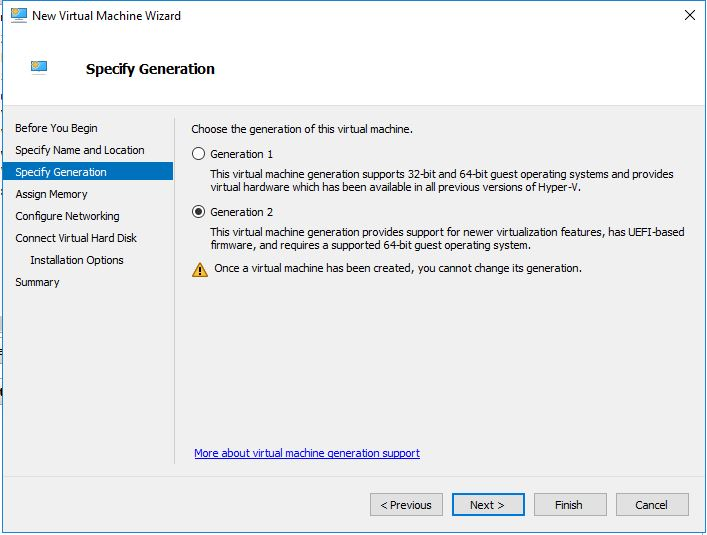
\includegraphics[width=0.8\textwidth]{generation_selection}
\caption{Generáció választás Hyper-V managerből készített virtuális gép esetén}
\label{fig:gen_selection}
\end{figure}


A másik irányzat amikor a Microsoft Deployment Toolkitet használjuk (továbbiakban MDT). Az MDT telljesen más felfogást követ. Itt light-touch megoldásról beszélünk, tehát lényegében egy automatizált telepítő végighalad azon a telepítési lépéseken amelyeket személyesen végigcsinálná a telepítést végző személy. 
Az MDT nagy előnye, hogy csak azokon a pontokon igényel interakciót, amelyeket nem tud magától meghatározni a rendszer, lehet ilyen az egyedi lokális adminisztártorok beállítása, a számítógép átnevezése. Az MDT telepítések, csoportházirenddel kombinálva közel ugyanazt a végeredményt érhetik el mint a master image-es megoldások. 

% TODO a különböző hardverek esetét kitárgyalni!

A két megoldás közötti legnagyobb különbség ám nem a végeredményben hanem a felhasznált időben rejlik. Az első megoldás esetén annyi időt kell a rendszer telljes beüzemelésére számítani amennyi idő alatt a közös helyről a VM konténer mappájába másolódik a VHDX, és a szükséges beállítások elvégzésre kerülnek. Ezzel szemben a második megoldás időigényesebb, mert ugyan felhasználó interakciót csak nagyon kevés ponton igényel, a telljes telepítési folyamatnak le kell zajlani mire használatba lehet venni a gépet. 

A szolgáltatók ezért inkább az első megoldást szokták választani. Könnyebb gyorsabb és kevesebb erőforrást igényel. Ha valami nagyon egyedit kér a felhasználó akkor lehet megoldást adni arra, hogy elérje a VM konzolját és így magának készíthesse el a telepítést.

\section{Automatizált megoldások}

\subsection{On-Premisess}


Az automatizált rendszer első és lefontosabb építőköve a gyors virtuális gépek elkészítése. Mivel az esettanulmányban egy szolgáltató céget tételeztem fel, így fontos volt, hogy minél kevesebb interakcióval, lehetőleg teljesen automatikusan lehessen legyártani az igényelt virtális gépeket. A virtulális gépek legyártása és managelése megoldható egy webfelületről.

\subsubsection{Provision-ObjectsForCompany.ps1}
Egy gyűjtő kód amely megfelelően paraméterezve elvégzni a telljes virtális gép létrehozás lépéseit. 
A következőkben taglalt scripteket hívja meg. 
A kódok végrehajtása az előkövetelményeknek megfelelően történik:
\begin{enumerate}
	\item Virtuális Switch létrehozása ( Crete-NewVirtualSwitch.ps1 )
	\item Viruális gép(ek) létrehozása ( Create-VM.ps1 )
	\item A virtális gépek hálózatba fűzése ( Set-VMSwitchForVM.ps1 )
\end{enumerate}

% \\TODO

\subsubsection{Create-NewVirtualSwitch.ps1}

Virtuális switchek tulajdonságát korábban taglaltam. A cégnél a megrendelők rendszerei teljesen elszerparált rendszerek, hacsak a megrendelők másképp nem rendelkeznek. Ellenben a virtuális gépek amelyek egy megrendelőhöz kötődnek egymással közös hálózaton vannak. Szolgáltatói oldalon a cégekhez tartozó erőforrások azonosítása érdekében a megrendelő cég nevét eléfűzöm az erőforrás nevéhez. Amennyiben már létezik ilyen erőforrás úgy a script küld egy email üzenetet az üzemeltetőnek, hogy manuális ellenőrzésre van szükség.

% \\TODO ?

\subsubsection{Create-VM.ps1}

A script egy az argumentumaiban szereplő paramétereknek megfelelő VM konténert hoz létre. A beállításokat tekintve, ha valamelyik paraméter nincs felülbírálva az argumentumokban, akkor a korábban már taglalt alapbeállítás kerül felhasználásra.

A script úgy lett elkészítve, hogy képes felismerni, ha valamelyik lemez VHDX állománya már létezik.


% \\TODO




\subsubsection{Post-Configuration.ps1}
% \\TODO

\subsubsection{Update-WebPage.ps1}
Mint azt már korábban említettem a rendszer működését egy weboldalon keresztül nyomon lehet követni. A webfelületnek van egy álltalános áttekintő nézete, amely a rendszeradminisztrátor számára ad egy képet pillanatnyi állásról. 
Biztonsági szempontokbólna a weblapot frissítő kódot nem olvashatja a cluster adatait, így a hostokról a webfelület számára fontos információkat a Get-HostStatistics.ps1 script gyűjti össze majd menti le egy olyan helyre amelyre van olvasási joga a jelenlegi scriptnek. Ezt az adatállományt dolgozza fel és vizualizálja. A webfelületen megjelenik az összes VM fontos tulajdonsága, a cluster kihasználtságára vonatkozó adatok, illetve a hostolt igénylők egymáshoz viszonyított erőforrásigénye.

A HTML kódot a Powershell XML modulján keresztül szerkesztem, a szükséges számításokat a frissítéskor számítja ki a script.

\subsubsection{Get-HostStatistics.ps1}
Biztonsági szempontból a weboldalt aktualizáló kódnak nincs még olvasási hozzáférése sem a clusterhez, ez a megoldás egyébként garantálja azt is, hogy mindegy hol van a világban a host vagy cluster, ha az a közös tárterületre képes az adatait lementeni beolvasztható a jelenlegi rendszerbe. 

Üzemeltetés szempontjából lényeges, hogy az adott gazdagépek processzora és memória készlete mennyire van kihasználva, ám még fontosabb információ a rendelkezésre álló tárterület. Éppen ezeket az információkat kérdezi le a script és tárolja le. Az adatokat a Powershell objektumokat exportálom XML fáljba, így megőrzök minden információt amelyet később vissza lehet nyerni a feldolgozás során.

\subsection{Cloud}
\noindent

\chapter{PowerShell}
A shell mint fogalom az informatikában a kezdetektől fogva létezik. A shell tulajdonképpen nem más, mint egy interfész amely lehetővé teszi a felhasználó és az operációs rendszer közötti interakciót. A shell lényegében nem egy alkalmazás a megkerülhetetlensége miatt, de nagyon hasonló bármely más folyamathoz a rendszerben. A shell-ek attól függően, hogy milyen operációs rendszeren találhatóak lehetnek parancssoros (UNIX, Linux, VMS) vagy grafikus interfészek (Windows vagy Mac OS X). Továbbiakban az angol terminológiából származtatott rövidítéseket fogom használni, a parancssoros felületre a Command-Line Interface azaz CLI-t, míg a grafikus interfészre a Graphical User Interface azaz GUI-t.

Mind a két shell-nek megvan az előnye és a hátránya. Az átlag felhasználó számára a GUI előnyösebb, mert nem igényel annyi előzetes tudást az adott rendszerrel kapcsolatban, elég ha a GUI-k általános használatát ismeri. Ebből kifolyólag nem a fejleszétsükkor nem volt szempont, hogy az egyik parancs kimenetét egy másik fel tudja dolgozni. 

A CLI-nek megvan az a nagy előnye, hogy a parancsok kiementeit egy másik parancs fel tudja dolgozni, ugyanakkor mivel parancssoros felülete van a felhasználónak mélyebb tudással kell rendelkeznie a használatához.

Habár léteznek GUI shell-ek, a shell-t mint fogalmat valamilyen CLI-re használják. Ugyanis a shell programozás is azt a cselekményt takarja amikor a megfelelő parancsok sokaságát összegyűjtjük amint egyébként a CLI-be táplálnánk vagy futtatható állományként átadnánk.
\cite{WindowsPowerShellUnleashed}

\subsubsection{A shell-ek története}
Az elsőkörben elterjedten használt shell a Bourne shell volt, amely a UNIX rendszerek alapértelmezett felhasználói felülete is egyben. C fejlesztőknek készítették C fejlesztők, ám mégsem C-szerű szintaxist használ. A Bourne shell egy robusztus megoldás volt amely képes volt csővezetékeket, feltételes és rekurzív szerkezeteket kezelni. A hiányosságai miatt elkészült a C shell-t, ez már tudott parancs aliaszokat, és parancssori szövegszerkesztőt. A korabeli shellek nagy problémája az volt, hogy rengeteget kellett képeni, hogy a kívánt eredményt megkapja a felhasználó. 
Időközben elkészült a Korn shell aminek a legnagyobb baja az volt, hogy megrendelésre készült és licensz köteles termék volt. Az ingyenes nyílt forráskódú rendszerek számára ez nem volt opció, így a Free Software Foundation égisze alatt megszületett a Bourne Again shell, röviden BASH.

A Microsoft korabeli rendszere a DOS volt. A DOS egyben shell és kernel is, ám tudásban bőven elmaradt a Bash-től. A Microsoft ezután bejelentette a Windows-t amely egy grafikus felhasználó interfész volt. A Windows megjelenésével együtt megérkezett a DOSShell szerű Command Promt (továbbiakban CMD). 
A CMD nem nyújtott elég nagy rugalmasságot a rendszerüzemeltetők számára, és a Microsoft is belátta ezt. Éppen ezért a Windows 98-ban beépítve érkezett a Windows Script Host-t (WSH). A WSH egy programkönyvtár volt amely lehetőséget adott a scripteknek a Windows alacsonyszintű vezérlésére.
A WSH legnagyobb előnye volt egyben a legnagyobb hátránya is. Nem volt egy egyértelműen meghatározott nyelve. Lehetett script-eket írni rá VBScript, JScript, Perl, Python, Kixstart és Object REXX nyelveken. Ugyan a nyelvet megválaszhatta a készítő a nyelvhez való környezetet már nem tartalmazta beépítve a Windows. Így nem lehetett garantálni, hogy ugyanaz a kód minden gépen futni fog. A WSH továbbá komoly veszélyforrás is volt, hiszen a scriptek hozzáfértek a Windows minden beállításához, tehát ha a vírusos kód már a gépen volt nem volt semmi ami megakadályozhatta volna a végrehajtódásban.

Mindezen lépések után a Microsoft végre elkészítette a PowerShell-t. A tervezésekor a legfontosabb szempontok a biztonság, a scriptelhetőség és a beépített nyelv voltak. A PowerShell alacsonyszintű hozzáféréssel rendelkezik a .NET Keretrendszeren, a Component Object Modellnek és társaiknak köszönhetően. Az egységessége és robusztusságának köszönhetően a mai napig a legjobb eszköz a rendszer üzemeltetők számára. A sikerét jól mutatja, hogy nem csak a Windows beállításait kezelni képes alap csomagok léteznek, hanem sok gyártó elkészítette a saját megoldásához a PowerShell modult, amelyen keresztül a menedzsment megoldható.
\cite{WindowsPowerShellUnleashed}

\subsubsection{PowerShell Veriótörténet és azok főbb újdonságai}
\noindent\textbf{PowerShell 1.0}
\newline 2003 Szeptemberében mutatták meg először a fejlesztőknek a Professional Developers Conference. 
Végül 2006 Novemberében megjelent a belépítve a következőkben Windows XP SP2, Windows Server 2003 SP1 és a Windows Vistaban. Opcionális komponensként pedig a Windows Server 2008-hoz is letölthető volt.\\
\break
\noindent\textbf{PowerShell 2.0}
\newline Az első komolyabb funkció csomagot a második főverzió már integrálásra került a Windows 7-be és a Windows Server 2008 R2-be. A Windows XP SP3, Windows Server 2003 SP2 és a Windows Vista SP1 is frissítette a gépre telepített PowerShell-t.
Ezzel a frissítéssel megjelent lényeges újjítások
\begin{itemize}
	\item \textbf{PowerShell remoting}: Innentől a Windows WS-Management szolgáltatásán keresztül meglehetett hívni egy script blockot vagy lehetett nyitni egy távoli powershell session-t és abban ugyanúgy dolgozni mintha a helyi gépen lenne.
	\item \textbf{Background jobs}: A powershell parancsokat, scripteket a háttérbe lehetett küldeni, amelyeknek ha van kimeneti értéke amelyet nem fájlba akartunk kimenteni, akkor a JobID-t ismerve a kimenetet vissza lehetett nyerni. Ezzel az aszinkron működést igénylő problémákat meg lehetett oldani. Amennyiben egy háttérben futó Job-nak input-ra volt szüksége, úgy annak a végrehajtását addig szüneteltette a rendszer, míg az input bevitelre nem kerül.
	\item \textbf{Tranzakciók}: A shell innentől alkalmas volt arra, hogy a parancsokat tranzakciós metodológia szerint dolgozza fel. Hasonlóan mint egy adatbáziskezelő rendszer. Ez a végrehajtási módszer szükséges lehet bizonyos Registy-t érintő módosításokra.
	\item \textbf{Modulok}: A kettes főverziótól bárkinek adott a lehetőség, hogy saját PowerShell modult írjon. A modulok lényegében parancsgyűjtemények. Leggyakrabban a nagyobb gyártók az alkalmazásaik egyszerűbb menedzsmentjéhez, vagy automatizálásához adnak ki ilyen modulokat. De az sem ritka, hogy nagyobb cégeknél az alkalmazottak által sűrűn használt egyedi scriptek, parancsokat egy modulba fogják össze és azt minden gépre szétszórják.
	\item \textbf{Script debugging}: A scriptek hibakeresésénél alapvető eszköz a brakepoint-ok lehetősége. Brakepointokat lehet hozzárendelni sorokhoz, sorokon belül oszlopokhoz, parancsokhoz, vagy akár egy változó értékének írásához, olvasásához.
	\item \textbf{Eseménykezelés}: A scriptek innentől hozzárendelhetőek Objektum, PowerShell és WMI eseményekhez, amelyekre a kód adhat választ valósidőben, vagy aszinkron módon.
	\item \textbf{Windows PowerShell Integrated Scripting Environment (ISE)}: A powershell scriptek készítése vagy nagyobb előzetes tudást igényelt, vagy időigényesebb volt, mert a parancsokat és azoknak a megfelelő kapcsolóit felhasználni nem egyszerű feladat. Az ISE tartalmazza belépítve az összes alap parancsot, szerkesztés közben kódkiegészítéssel és a kapcsolók felajánlásával segíti a felhasználót. Mindezek mellett még szintakszis kiemelést is tartalmaz. Az ISE nagy előnye még hogy a script egyes részeit a beépített konzolon egyből le is lehet futtatni. Ezekből a konzolokból egyszerre maximum 8-at lehet nyitvatartani. 
	\item \textbf{Network File Transfer}: Out-of-the-Box módon támogatja a BITS fájlátvitelt az eszközök között aszinkron módon.
	\item \textbf{Out-GridView}: Amennyiben az eredményt, nem az alap karakteres felületen megjelenő módon szeretnénk közölni, van lehetőség a .NET keretrendszer álltal adott WPF GridView-ben ablakban megjeleníteni, amely beépítetten tartalmaz szűrés és rendezés funkciókat, és a végső eredményt le is menthetjük a grafikus felületről is.
	\item \textbf{Kivételkezelés}: A scriptekben a kivétgelkezelés során a catch ágakon belül egyszerre több különböző kivétel tipust is le lehet kezelni, és létezik finally ág is, ha végképp váratlan típusú esmény következett volna be. 
	\item \textbf{Block comments}: Innetől lehetőség van blokkokban kommenteket elhelyezni, illetve in-line kommentelésre is. 
	\item \textbf{Split, Join, @}: Az adatállományokat főként a \textit{String} típust kezelő utasítások közé bekerült a Split és a Join amely tömbelemeket tudott feldarabolni vagy összefűzni. A @ operátorral pedig üres tömböt, lehet létrehozni.
\end{itemize}

\break
\noindent\textbf{PowerShell 3.0}
\newline Beépítve érkezett a Windows 8 és Windows Server 2012 operációs rendszerekben, ugyanakkor letölthető formátumban telepíthető volt a Windows 7 SP1, Windows Server 2008 SP1 és Windows Server 2008 R2 SP1 rendszerekre is. 
A PowerShell 3.0 már nem ölállóan érkezett hanem egy nagyobb csomag a Windows Management Framework 3.0 részekét. A WMF3 magában hordozta a WinRM-et is, amelly a megnövelt tudású távoli vezérlést tette lehetővé.
\begin{itemize}
	\item \textbf{Scheduled jobs}: Ettől a verziótól a PowerShell jobokat már lehetett üzemezni.
	\item \textbf{Session connectivity}: A PowerShell session-ök érzékenyek voltak a lassú, vagy szakadozó hálózatra. A frissítés után a session-ök folytathatóvá válltak ezzel megoldva az instabil hálózat okozta gondokat.
	\item \textbf{Improved code writing}: A ISE-t érintette egy kisebb ráncfelvarrás, innentől elérhetővé váltak a párbeszéd ablakok, az előre nem megadott, de kötelező értékkel rendelkező paraméterek beadására. Továbbá bekerültek a snippetek és a kódkiegészítés is sokat javult.
	\item \textbf{Delegálás}: Adminisztratív feladatokat powershell-en keresztül ki lehetett delegálni olyan felhasználóknak akiknek egyébként nincs megfelelő jogkörük a feladat végrehajtásához. 
	\item \textbf{Frissíthető help}: A parancsok és scriptek segítség szekcióját most már a shell ablakból lehetett frissíteni, így nem kellett megvárni az újabb kiadását a shell-nek a frissítésekért.
	\item \textbf{Automatikus modul detektálás}: A korábbi PowerShell verziókban ha egy olyan modulból szeretett volna parancsot hívni a script vagy a felhasználó amely nem az alapcsomag része, akkor azt kézzel Import-Module paranccsal be kellett tölteni a munkamenetbe és csak azután lehetett használni a tartalmát. Azonban a 3.0 főverziótól kezdve, amennyiben a modul telepítve van a shell automatikusan betölti amint az első parancs meghívásra kerül belőle.
	\item \textbf{Új parancsok}: A Microsoft folyamatosan bővítette a parancsokat amelyekkel a rendszert lehet üzemeltetni. Ezzel a frissítéssel a lemezek, meghajtók kezelésére, a tűzfal és hálózati kapcsolatok beállításának a módosítására és nyomtató menedzsmentre alkalmas parancsok jelentek meg. Ez nagy segítség volt, mert korábban ezeket a beállításokat WMI-on keresztül lehetett elérni. 
\end{itemize}

\noindent\textbf{PowerShell 4.0}
\newline A Windows 8.1 és Windows Server 2012 R2-es rendszerekbe beépítve debütált. Természetesen minden korábbi még támogatott Operációs rendszer legfrissebb Service Pack-es verziójára telepíthető volt.

\begin{itemize}
	\item \textbf{Új házirend}: A PowerShell már a kezdetetkől fogva tartalmazott házirendeket a scriptek futtatásának a korlátozására. A négyes főverziótól kezdve a minimális szint alapértelmezésként, egy távoli számítógép (Domain Controller) álltal aláírt script. Ettől a beállítástól természetesen el lehet térni, ha a felhasználó nem akar minden saját készítésű scriptet aláíratni.
	\item \textbf{-PipelineVariable kapcsoló}: A csővezetékek kezelése során előfordulhat, hogy valamelyik átadáskori adatállapotot, egy változóban szeretnénk tárolni a későbbi adatmanipuláció vagy feldolgozás végett. Erre adott lehetőséget ez az újdonsága.
	\item \textbf{Új Hyper-V parancsok}: Többek között most már a Virtuális Switcheket is lehet a shellből kezelni. Ennélkül a funkció nélkül az én dolgozatomban található scriptek sem működnének.
	\item \textbf{Szűrés és iterációk}: 4.0-tól elérhetővé vált a ciklusoknál a ForEach, amely egy Iterable típusú elemcsoport minden elemét képes bejárni. Ezáltal nagyban megkönnyítve a készítő dolgát, továbbá javítva a scriptek olvashatóságát.
\end{itemize}

\noindent\textbf{PowerShell 5.0 és 5.1}
\newline Az 5.0 csak letölthető formában létezett a Windows 10-et kivéve amelybe beépítésre került. Az igazi újdonságot azonban az 5.1-es verzió hozta, amely bejelentésekor két külön ágazat jelent meg. Desktop és a Core verzió. A Desktop verzió a szabványos .NET keretrendszerre épül és beépítve megtalálható a Windows 10 Anniversary Update-ben és Windows Server 2016 Core, Standard, és Datacenter kiadásaiban. Míg a PowerShell Core, a Nano Server-be van előre telepítve. Ez az irányvonal az eleve csökkentett képességű célirányosan létrehozott operációs rendszerhez passzol, csak azok a modulok érhetőek el amelyek a csökkentett utasításkészlethez szükségesek és tartalmazza a .NET Core verzióját is amely tökéletesen elég minden a Nano Server által támogatott szolgáltatásnak.\\


\noindent\textbf{PowerShell 6.0}
\newline A dolgozat készítésekor még nem található beépített módon egyik rendszerben sem. Azonban elérhető minden támogatott Windows Operációs rendszer mellett, macOS-re és UNIX-ra is. Ez az első lépése a Microsoftnak affelé, hogy egy közös menedzsment platformot hozzon létre. Ami kicsit meglepő az eddigi termékpolitikát tekintve, hogy a nem microsoft rendszerekre is ingyenesen elérhető.
A cross-platform management témakörét ugyan nem most veszi elő a Windows először, hiszen a Windows 10-től ugyan még Beta státuszban de a Bash is elérhető a Microsoft rendszerét futtató gépekre, amennyiben az kilép a fejlesztési státuszból a Shell emulátorokat végre fel lehet számolni.

\section{Programozási paradigmák}

asd
% \\TODO
\cite{PowerShellGuidelines}

\addcontentsline{toc}{chapter}{\listfigurename}
\listoffigures
\printbibliography[heading=bibintoc,title={Irodalomjegyzék}]
\end{document}
